\begin{center}
    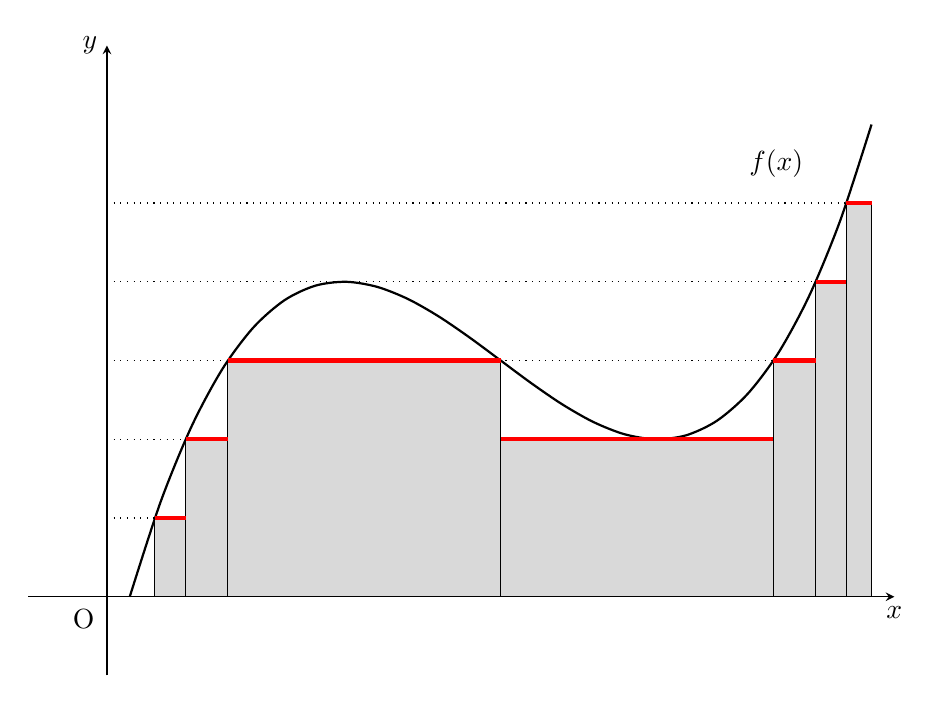
\begin{tikzpicture}[
            simple/.style={red, ultra thick},
            dots/.style={thin, dotted},
            rect/.style={fill=gray!30, draw=black},
        ]
        \node[below left=1pt] (origin) at (0,0) {\(\rm{O}\)};
        \draw [-stealth] (-1, 0) -- (10, 0) node[below] {\(x\)};
        \draw [-stealth] (0, -1) -- (0, 7) node[left] {\(y\)};

        \draw[dots] (0, 1) -- (0.6083, 1);
        \draw[dots] (0, 2) -- (1, 2);
        \draw[dots] (0, 3) -- (8.4641, 3);
        \draw[dots] (0, 4) -- (9.3916, 4);
        \draw[dots] (0, 5) -- (9.7106, 5);

        \draw[thick,domain=0.2893:9.71, smooth, variable=\x] plot ({\x}, {-3.0625 + 3.9375*\x - 0.9375*\x^2 + \x^3/16 + 2});

        \pgfmathsetmacro{\maxn}{3}
        \pgfmathsetmacro{\limit}{24}

        \filldraw[rect] (0.6083, 1) rectangle (1, 0);
        \filldraw[rect] (1, 2) rectangle (1.5358, 0);
        \filldraw[rect] (1.5358, 3) rectangle (5, 0);
        \filldraw[rect] (5, 2) rectangle (8.4641, 0);
        \filldraw[rect] (8.4641, 3) rectangle (9, 0);
        \filldraw[rect] (9, 4) rectangle (9.3916, 0);
        \filldraw[rect] (9.3916, 5) rectangle (9.7106, 0);

        \draw[simple] (0.6083, 1) -- (1, 1);
        \draw[simple] (1, 2) -- (1.5358, 2);
        \draw[simple] (1.5358, 3) -- (5, 3);
        \draw[simple] (5, 2) -- (8.4641, 2);
        \draw[simple] (8.4641, 3) -- (9, 3);
        \draw[simple] (9, 4) -- (9.3916, 4);
        \draw[simple] (9.3916, 5) -- (9.7106, 5);

        \node at (8.5, 5.5) {\(f(x)\)};
    \end{tikzpicture}
\end{center}

\section*{Lebesgue Integration}

르벡 적분을 단계적으로 정의하려고 합니다. \(X = (X, \scr{F}, \mu)\) 라고 계속 가정합니다. \(\scr{F}\)는 \(\sigma\)-algebra on \(X\), \(\mu\)는 \(\scr{F}\)의 measure 입니다.

\(E \in \scr{F}\) 일 때, 적분을 정의하기 위해
\[
    \scr{F}_E = \{A \cap E : A \in \scr{F}\}, \quad \mu_E = \mu|_{\scr{F}_E}
\]
로 설정하고 \(\int = \int_E\) 로 두어 (\(X, \scr{F}_E, \mu_E\)) 위에서 적분을 정의할 수 있습니다. 그러나 굳이 이렇게 하지 않아도 됩니다. \(\int = \int_X\) 로 두고
\[
    \int_E f \d{\mu} = \int f \chi _E \d{\mu}
\]
로 정의하면 충분하기 때문입니다. 이제 르벡 적분을 다루기 위해 simple function부터 적분해보겠습니다. 우선 가장 간단한 characteristic function부터 단계를 밟아나가야 합니다.

\textbf{\sffamily (Step 1)} \(A \in \scr{F}\) 에 대하여
\[
    \int \chi_A \d{\mu} = \mu(A)
\]
로 정의한다.

함수 \(\chi_A\)는 \(x \in A\) 일 때만 함숫값 \(1\)을 갖고 이외의 경우에는 \(0\)이기 때문에 이 함수를 \(X\) 위에서 적분하면 `\(A\)의 길이'에 대응되는 \(\mu(A)\)가 결과인 것이 자연스럽습니다.

다음으로 양의 값을 갖는 measurable simple function에 대해 정의합니다. \(f = f^+ - f^-\) 에서 \(f^+, f^-\) 모두 양의 값을 갖기 때문에 양의 값에 대해 먼저 정의합니다.

\textbf{\sffamily (Step 2)} \(f: X \ra [0, \infty)\) 가 measurable simple function이라 하자. \\
그러면 \(A_k \subset \scr{F}\) 이면서 쌍마다 서로소인 집합열 \(\seq{A_k}_{k=1}^n\)과 \(a_k \in [0, \infty)\) 인 수열 \(\seq{a_k}_{k=1}^n\)을 잡아
\[
    f(x) = \sum_{k=1}^n a_k \chi_{A_k}
\]
와 같이 표현할 수 있다. 이제
\[
    \int f\d{\mu} = \sum_{k=1}^n a_k \mu(A_k) \in [0, \infty]
\]
로 정의한다.

Measurable simple function은 measurable characteristic function의 linear combination으로 표현할 수 있기 때문에, 이와 같은 정의를 생각할 수 있습니다. 하지만 이런 정의를 보면 well-definedness를 제일 먼저 생각해야 합니다. 위와 같은 linear combination 표현이 유일하지 않기 때문입니다.

Well-definedness를 증명하기 위해 임의의 linear combination을 잡아도 적분값이 항상 같음을 보이면 됩니다.

\prop. 위 정의는 모든 measurable simple function에 대해 well-defined이다.

\pf \(f\)가 다음과 같이 두 가지 방법으로 표현된다고 하자.
\[
    f(x) = \sum_{k=1}^n a_k \chi_{A_k} = \sum_{i=1}^m b_i \chi_{B_i}.
\]
여기서 \(k = 1, \dots, n\), \(i = 1, \dots, m\) 에 대하여 \(0\leq a_k, b_i < \infty\) 이고 \(A_k, B_i \in \scr{F}\) 이다. 여기서 \(A_k, B_i\)는 각각 쌍마다 서로소로, \(X\)의 분할이 된다. \(C_{k, i} = A_k \cap B_i\) 로 두면
\[
    \sum_{k=1}^n a_k \mu(A_k) = \sum_{k=1}^n a_k \mu\paren{A_k \cap \bigcup_{i=1}^m B_i} = \sum_{k=1}^n \sum_{i=1}^m a_k \mu(C_{k, i}),
\]
\[
    \sum_{i=1}^m b_i \mu(B_i) = \sum_{i=1}^{m} b_i \mu\paren{B_i \cap \bigcup_{k=1}^n A_k}= \sum_{i=1}^m \sum_{k=1}^n b_i \mu(C_{k, i})
\]
이다. 이 때 \(C_{k, i} \neq \varnothing\) 이면 \(x \in C_{k, i}\) 에 대해 \(f(x) = a_k = b_i\) 가 된다. 한편 \(C_{k, i} = \varnothing\) 이면 \(\mu(C_{k, i}) = 0\) 이다. 이로부터 모든 \(k, i\)에 대하여 \(b_i \mu(C_{k, i}) = a_k \mu(C_{k, i})\) 임을 알 수 있다.\footnote{계수가 같거나, measure가 0이 되어 같거나.} 따라서
\[
    \int f \d\mu = \sum_{k=1}^n a_k \mu(A_k) = \sum_{i=1}^m b_i \mu(B_i)
\]
가 되어 적분값은 유일하고 위 정의가 well-defined임을 알 수 있다.

이제 measurable simple function은 얼마든지 적분할 수 있습니다. 이제 다음은 measurable function으로 확장할 단계입니다. 확장을 편하게 하기 위해 약간의 준비 작업을 거치겠습니다.

적분은 선형이고, monotonicity를 항상 유지하기를 기대합니다. 아직은 함수가 \(0\)보다 클 것을 가정했기 때문에 이를 계속 활용합니다.

\rmk \(a, b \in [0, \infty)\) 와 measurable simple function \(f, g \geq 0\) 에 대하여
\[
    \int \paren{af + bg} \d{\mu} = a \int f \d{\mu} + b \int g \d{\mu}
\]
이다.

\pf 위 Step 2와 동일하게
\[
    f = \sum_{j=1}^m y_j \chi_{A_j}, \quad g = \sum_{k=1}^n z_k \chi_{B_k}
\]
로 둘 수 있다. 여기서 \(A_j, B_k\)는 \(X\)의 분할이고 \(y_j, z_k \geq 0\) 이다. 마찬가지로 \(C_{j, k} = A_j \cap B_k\) 로 정의하면
\[
    \begin{aligned}
        a \int f \d{\mu} + b \int g \d{\mu} & = \sum_{j} ay_j \mu(A_j) + \sum_k b z_k \mu(B_k)                                 \\
                                            & = \sum_{j} ay_j \sum_k \mu(A_j \cap B_k) + \sum_k b z_k \sum_j \mu(B_k \cap A_j) \\
                                            & = \sum_{j} \sum_k ay_j \mu(C_{j, k}) + \sum_k \sum_j b z_k \mu(C_{j, k})         \\
                                            & = \sum_{j, k} (ay_j + bz_k) \mu(C_{j, k}) = \int \paren{af + bg} \d{\mu}
    \end{aligned}
\]
이다.

\rmk \(f \geq g \geq 0\) 이 measurable simple function일 때,
\[
    \int f \d{\mu} \geq \int g \d{\mu}
\]
이다.

\pf \(f - g \geq 0\) 이 simple이고 measurable임을 활용한다.
\[
    \int f \d{\mu} = \int \left[g + (f - g)\right] \d{\mu} = \int g\d{\mu} + \int (f - g) \d{\mu} \geq \int g \d{\mu} \geq 0.
\]

위와 같이 \(g + (f-g)\) 로 변형해야 하는 이유는 \(g\)의 적분값이 무한대인 경우 이를 이항할 수 없기 때문입니다. 하지만 \(f-g\) 의 적분값이 \(0\) 이상인 것은 확실하게 알 수 있습니다.

이제 양의 값을 가지는 임의의 measurable function을 고려해 보겠습니다.

\textbf{\sffamily (Step 3)} \(f: X \ra [0, \infty]\) 가 measurable일 때,
\[
    \int f \d{\mu} = \sup\left\{\int h \d{\mu}: 0\leq h \leq f, h \text{ measurable and simple}\right\}.
\]
로 정의한다.

\(f\)보다 작은 measurable simple function의 적분값 중 상한을 택하겠다는 의미입니다. \(f\)보다 작은 measurable simple function으로 \(f\)를 근사한다고도 이해할 수 있습니다. 또한 \(f\)가 simple function이면 Step 2의 정의와 일치하는 것을 알 수 있습니다.

\(f \geq 0\) 가 measurable이면 증가하는 measurable simple 함수열 \(s_n\)이 존재함을 지난 번에 보였습니다. 이 \(s_n\)에 대하여 적분값을 계산해보면
\[
    \int_E s_n \d{\mu} = \sum_{i=1}^{n2^n} \frac{i - 1}{2^n}\mu\paren{\left\{x \in E : \frac{i-1}{2^n} \leq f(x) \leq \frac{i}{2^n}\right\}} + n\mu(\{x \in E : f(x)\geq n\})
\]
임을 알 수 있습니다. 이제 \(n \ra \infty\) 일 때 우변이 곧 \(\ds \int f \d{\mu}\) 이기를 기대합니다.

위 내용에 대한 증명은 추후 다루도록 하고 식의 의미를 이해해 보겠습니다. \textbf{르벡 적분은 치역을 잘게 잘라} 자른 치역 부분의 preimage에 대해 measure를 사용하여 길이를 잽니다. 그리고 함숫값과 preimage의 measure를 곱한 뒤 더해 넓이를 계산한다고 이해할 수 있습니다. \textbf{리만 적분은 정의역을 잘게 잘라} 상합/하합을 고려하여 정의한 것과는 다른 접근 방법입니다.

이제 마지막 단계입니다. 임의의 measurable function에 대해 정의합니다.

\textbf{\sffamily (Step 4)} \(f\)가 measurable이면 \(f^+, f^- \geq 0\) 도 measurable이다. 그러므로 \(E \in \scr{F}\) 에 대하여
\[
    \int_E f \d{\mu} = \int_E f^+ \d{\mu} - \int_E f^- \d{\mu}
\]
와 같이 정의한다. 단, 우변에서 \(\infty - \infty\) 가 등장하는 경우는 제외한다.

우변에서 \(\infty - \infty\) 인 경우는 제외되었기 때문에 \(f^+\), \(f^-\)의 적분값 둘 중 하나는 유한해야 합니다.

위 내용을 종합하여 다음 정의를 얻습니다.

\defn. \note{르벡 적분 가능} \(f\)가 measurable이고,
\[
    \int_E \abs{f} \d{\mu} = \int_E f^+ \d{\mu} + \int_E f^- \d{\mu} < \infty
\]
이면 \(f\)가 \(E\)에서 \(\mu\)에 대해 \textbf{르벡 적분 가능}하다고 한다.

\notation \(f\)가 \(E\)에서 \(\mu\)에 대해 르벡 적분 가능하면
\[
    f \in \mc{L}^1(E, \mu)
\]
로 표기한다. 특별히 \(\mu = m\) 이면 \(f \in \mc{L}^1(E)\) 로 적는다.

즉 다음이 성립합니다.
\[
    f \in \mc{L}^{1}(E, \mu) \iff f^+, f^- \in \mc{L}^{1}(E, \mu)\iff \abs{f} \in \mc{L}^{1}(E, \mu).
\]

\dots

다음 글에서는 르벡 적분의 성질과 수렴 정리에 대해 다루도록 하겠습니다.

\pagebreak
